\documentclass[11pt,twocolumn]{article}

\usepackage[letterpaper,margin=0.66in,columnsep=0.24in]{geometry}
\usepackage[T1]{fontenc}
\usepackage{lmodern}
\usepackage{microtype}
\usepackage{graphicx}
\usepackage{booktabs}
\usepackage{array}
\usepackage{xcolor}
\usepackage{enumitem}
\usepackage{caption}
\usepackage{amsmath}
\usepackage{amssymb}
\usepackage{hyperref}
\usepackage{float}
\usepackage{titlesec}

\graphicspath{{figures/}}
\hypersetup{colorlinks=true,linkcolor=blue!45!black,citecolor=blue!45!black,urlcolor=blue!45!black}
\captionsetup{font=small,labelfont=bf}
\setlength{\parindent}{0.9em}
\setlength{\parskip}{0.04em}
\setlist[itemize]{leftmargin=1.05em,itemsep=0.02em,topsep=0.04em}
\renewcommand{\arraystretch}{1.03}
\raggedbottom
\titlespacing*{\section}{0pt}{0.55em}{0.25em}

\title{\vspace{-1.8em}\textbf{PatchTST: a Case Study on Electricity Forecasting}}
\author{CS 5782 Deep Learning Final Project, Zhihan Liu }
\date{}

\begin{document}
\twocolumn[
\maketitle
%\vspace{-2.0em}
\begin{center}
%\begin{minipage}{0.94\textwidth}
%\textbf{Abstract.}
%PatchTST is a Transformer-based architecture for long-term time-series forecasting that represents each univariate series as a sequence of subseries-level patch tokens and applies a shared encoder independently across channels. In this project, we reproduce the PatchTST/64 result on the Electricity dataset for prediction horizon $H=96$, then extend the experiment with masked-patch self-supervised learning (SSL) pretrain and a scale-sensitivity probe. Our supervised reproduction nearly matches the paper's reported Electricity-96 MSE, and our SSL variants improve the test MSE in this setting. The scale probe shows that performance degrades in a step-like pattern under temporal coarse-graining, suggesting that the learned representation is structured around particular temporal resolutions rather than fully scale-invariant.
%\end{minipage}
\end{center}
%\vspace{0.15em}
]

\section{Introduction}

Time-series forecasting predicts future values over a target horizon. Longer lookback windows can capture seasonal patterns, delayed dependencies, and slow trends, but point-level Transformer tokens are inefficient: individual timestamps are low-context and potentially noisy, while neighbouring timestamps are often redundant. PatchTST \cite{nie2023patchtst} addresses this by replacing point tokens with subseries-level patch tokens and using channel independence. Each univariate series is split into local segments, so one token represents a short temporal shape rather than a single value, and shared Transformer weights are applied independently across channels.

If the input length is $L$, patch length is $P$, and stride is $S$, the number of patch tokens is
\begin{equation}
N = \left\lfloor \frac{L-P}{S} \right\rfloor + 2 \approx \frac{L}{S}.
\label{eq:patch_count}
\end{equation}
Thus the attention-map cost changes from roughly $O(L^2d)$ for point-level tokens to $O(N^2d)$ for patch-level tokens, with an additional patch-projection cost of $O(NPd)$. Patching therefore makes longer historical context more practical while preserving local values inside each segment.

In this project, we reproduce supervised PatchTST/64 on Electricity with prediction horizon $H=96$, implement the paper-aligned random-masking SSL+FT setting, and add a block-masking SSL variant that masks contiguous temporal regions. We also include a scale-sensitivity probe: because patch tokens encode local temporal segments, we evaluate trained models on coarse-grained inputs to test whether the learned representation is stable under changes in temporal resolution. This diagnostic is separate from final forecasting MSE and is defined in \eqref{eq:scale_ratio} and visualized in \autoref{fig:scale_sensitivity}.



\section{Chosen Result}

Our primary chosen result is the supervised PatchTST/64 result on Electricity with prediction horizon $H=96$, reported in Table 3 of Nie et al. as MSE $0.129$ and MAE $0.222$ \cite{nie2023patchtst}. This row is a meaningful reproduction target because Electricity is one of the paper's large multivariate benchmarks: it contains 321 electricity-consumption channels and 26,304 timesteps, and the authors group it with Weather and Traffic as larger datasets where results are more stable and less susceptible to overfitting. It is also directly connected to PatchTST's main design claims. Patching must preserve useful temporal structure over a long input window, while channel independence must work across many related customer-level series. The relevant architectural reference is the paper's Figure 1, reproduced in \autoref{fig:paper_architecture}, which shows channel-independent patching, a shared Transformer backbone, and forecasting or reconstruction heads.

We chose the Electricity-96 setting because it is concrete, computationally feasible for a course project, and necessary for interpreting our extensions. If our supervised PatchTST/64 baseline were far from the paper's result, then the SSL gains in \autoref{fig:forecasting_gain} would be hard to attribute to masked-patch pretraining rather than implementation mismatch. As a secondary reference, Table 4 of the paper reports an SSL fine-tuning result on Electricity-96 with MSE $0.126$ and MAE $0.221$ \cite{nie2023patchtst}. 





\section{Methodology}

\textbf{Data.} We use the UCI Electricity \cite{electricity} load dataset with chronological train, validation, and test splits. 

\textbf{Supervised PatchTST.} For the main reproduction, we use the PatchTST/64 setting summarized in \autoref{tab:complete_results}:
\[
L=512,\qquad H=96,\qquad P=16,\qquad S=8.
\]
This gives $N=64$ patch tokens by \eqref{eq:patch_count}. Each channel is instance-normalized, patchified, projected to $d=128$, given a learned positional embedding, reshaped to $(B\cdot C)\times N\times d$, and encoded by a shared Transformer. The encoder uses 3 layers, 16 heads, BatchNorm residual blocks, dropout $0.2$, feed-forward width 512, and a flatten-linear forecasting head. The forecast is predicted in normalized coordinates and then rescaled to the original input scale. Our code and repository are available in \cite{Repo}.

\textbf{Implementation choices.} Our implementation follows the PatchTST architecture at the level of the modeling idea. The supervised PatchTST/64 reproduction uses an end-padded tokenizer: the final input value is repeated by one stride before unfolding, matching the $N=64$ patch count for $L=512,P=16,S=8$. In contrast, the paper-aligned SSL runs use a no-extra-padding tokenizer with $P=12,S=12$, producing 42 non-overlapping patches from the last 504 points of the 512-point input window. Thus, the supervised and SSL experiments share the same PatchTST-style encoder design and per-window instance normalization, but not the same patch granularity or padding convention.

\textbf{SSL and fine-tuning.} Masked SSL trains the encoder to reconstruct normalized target patches. During pretraining, selected patch tokens are replaced by a learned mask token, and a reconstruction head predicts the original normalized patch values; the SSL loss is MSE over masked patches only. After pretraining, we attach the forecasting head and fine-tune end to end on Electricity-96. Random masking is closest to the paper's masked-patch SSL setup. Block masking is our extension: it masks contiguous temporal patch regions rather than independently selected patches, testing whether reconstructing missing time blocks gives a different forecasting representation.

\textbf{Scale probe.} To test the coarse-graining hypothesis, we transform the input by a temporal scale $\lambda=e^s$, resize it back to length 512, and evaluate without retraining. We report
\begin{equation}
\label{eq:scale_ratio}
r(\lambda)=
\frac{\mathrm{MSE}\bigl(f_\theta(T_\lambda x),y\bigr)}
{\mathrm{MSE}\bigl(f_\theta(x),y\bigr)},
\end{equation}
where $T_\lambda$ is the coarse-graining-and-resizing operator. Values near 1 indicate robustness; larger values indicate degradation.


\section{Results and Analysis}
The supervised reproduction is the anchor result. As shown in \autoref{fig:forecasting_gain} and \autoref{tab:complete_results}, our PatchTST/64 run obtains MSE $0.1294$, compared with the paper's MSE $0.1290$. The gap is small relative to the baselines in the same figure, so we regard the reproduction as successful for the purpose of analysis. It also suggests that the essential ingredients are implemented correctly. Remaining discrepancies could come from exact padding, scheduler details, random seed, or preprocessing conventions.


Block SSL+FT achieved the best MSE in our runs, slightly improving over Random SSL+FT even though it used a shorter fine-tuning schedule, 10 epochs rather than 15. This makes block masking a promising extension: reconstructing contiguous missing regions may encourage the encoder to learn more coherent temporal representations. However, the numerical gap is small, and the fine-tuning budgets are not identical, so we do not claim that block masking is definitively better. A fairer comparison would match the fine-tuning schedule across masking strategies or report multiple seeds with validation-based early stopping.

The scale-sensitivity experiment in \autoref{fig:scale_sensitivity} probes a different property from benchmark MSE. Both PatchTST/64 and SSL+FT degrade as the coarse-graining level increases. The degradation is also step-like rather than smooth, suggesting that the representations learned by the model are clustered around certain characteristic scales. 



\section{Reflections}


Our results match the the paper's Electricity-96 result overall, suggesting a reasonable PatchTST implementation. 

The SSL results were encouraging but not conclusive. Both random SSL+FT and block SSL+FT improved over our supervised PatchTST/64 run, and block masking achieved the best MSE with fewer fine-tuning epochs than random masking. This suggests that reconstructing contiguous missing regions may encourage more useful temporal representations. However, the gap is small and the fine-tuning budgets were not identical, so a stronger comparison would require matched schedules, multiple seeds, and validation-based early stopping.

The scale-sensitivity probe asked a different question from final MSE. After coarse-graining the input, the error increased in a step-like pattern, suggesting that the learned patch representations are not scale-invariant but clustered around certain characteristic scales. Because coarse-graining and resizing may introduce artifacts, this result should be viewed as exploratory. We hope to probe the representations learned directly and study the scale distribution of them in the future.

 

\vspace{-0.3em}
\begin{thebibliography}{9}\scriptsize
\setlength{\itemsep}{0.05em}
\bibitem{nie2023patchtst} Y. Nie et al. \textit{A Time Series Is Worth 64 Words: Long-term Forecasting with Transformers}. ICLR, 2023. \url{https://arxiv.org/abs/2211.14730}.
\bibitem{electricity} A. Trindade. \textit{ElectricityLoadDiagrams20112014}. UCI Machine Learning Repository, 2015.
\bibitem{pytorch} A. Paszke et al. \textit{PyTorch}. NeurIPS, 2019.
\bibitem{Repo} Z. Liu. \textit{PatchTST Electricity Re-implementation Repository}. GitHub, 2026. \url{https://github.com/KrasusZL/5782-Final-Project}.
\end{thebibliography}

\clearpage
\onecolumn
\section*{Visual Appendix}
\vspace{-1.1em}
\captionsetup{font=footnotesize,labelfont=bf}
\begin{figure}[H]
\centering
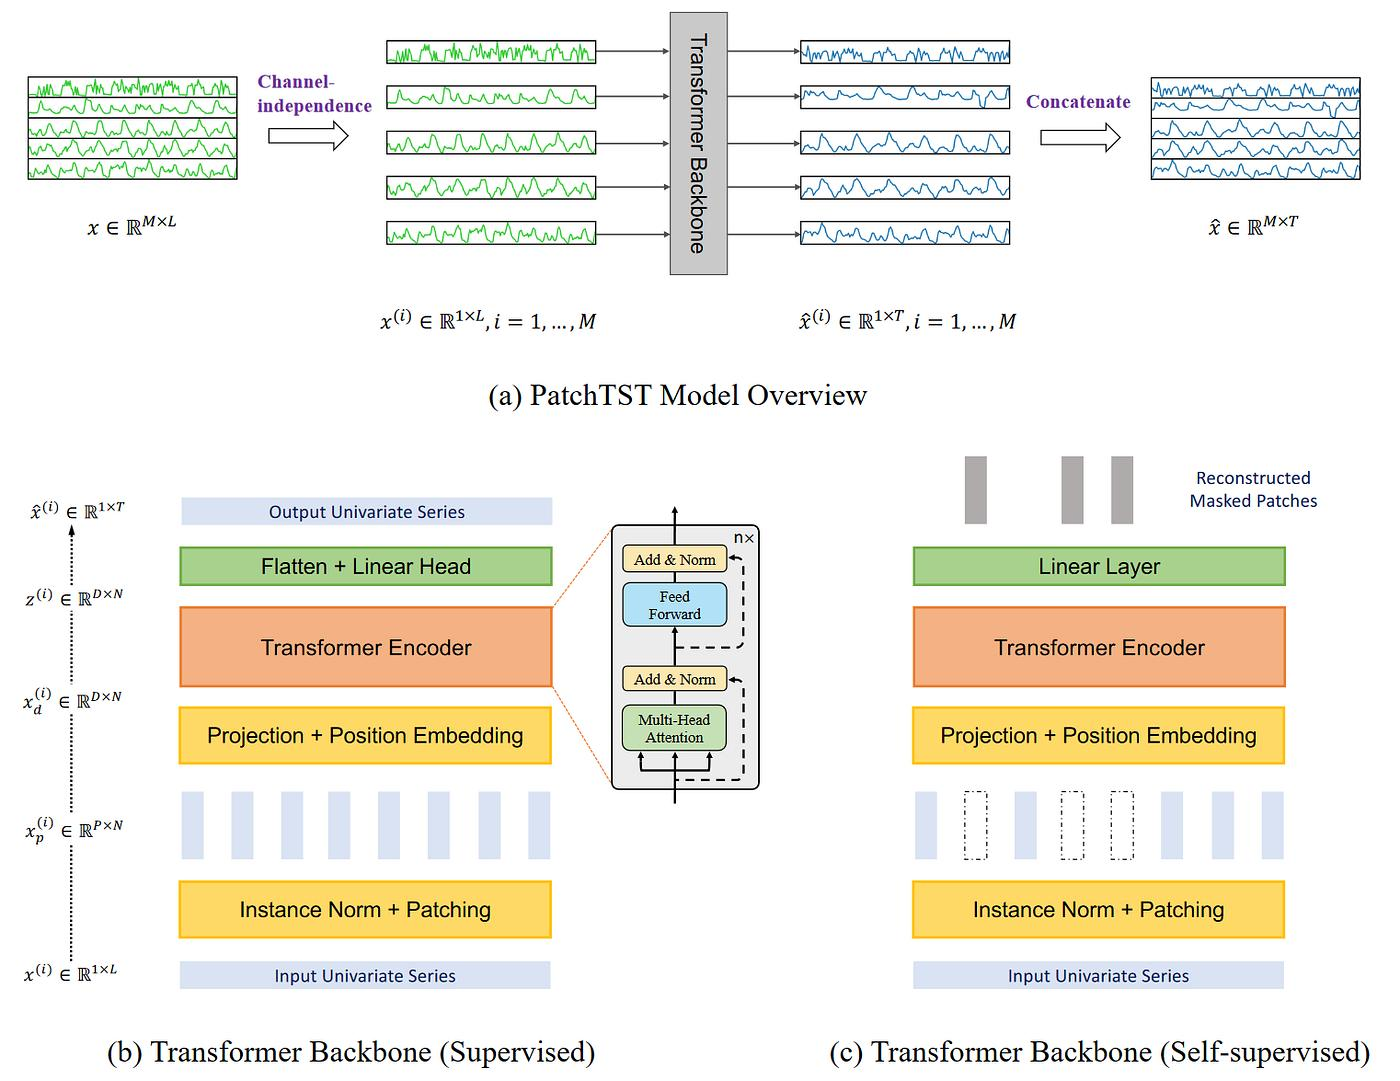
\includegraphics[width=0.60\textwidth]{patchtst_paper_figure1.jpeg}
\caption{PatchTST architecture, reproduced from Nie et al., Figure 1 \cite{nie2023patchtst}.}
\label{fig:paper_architecture}
\end{figure}
\vspace{-1.4em}

\begin{figure}[H]
\centering
\begin{minipage}{0.485\textwidth}
\centering
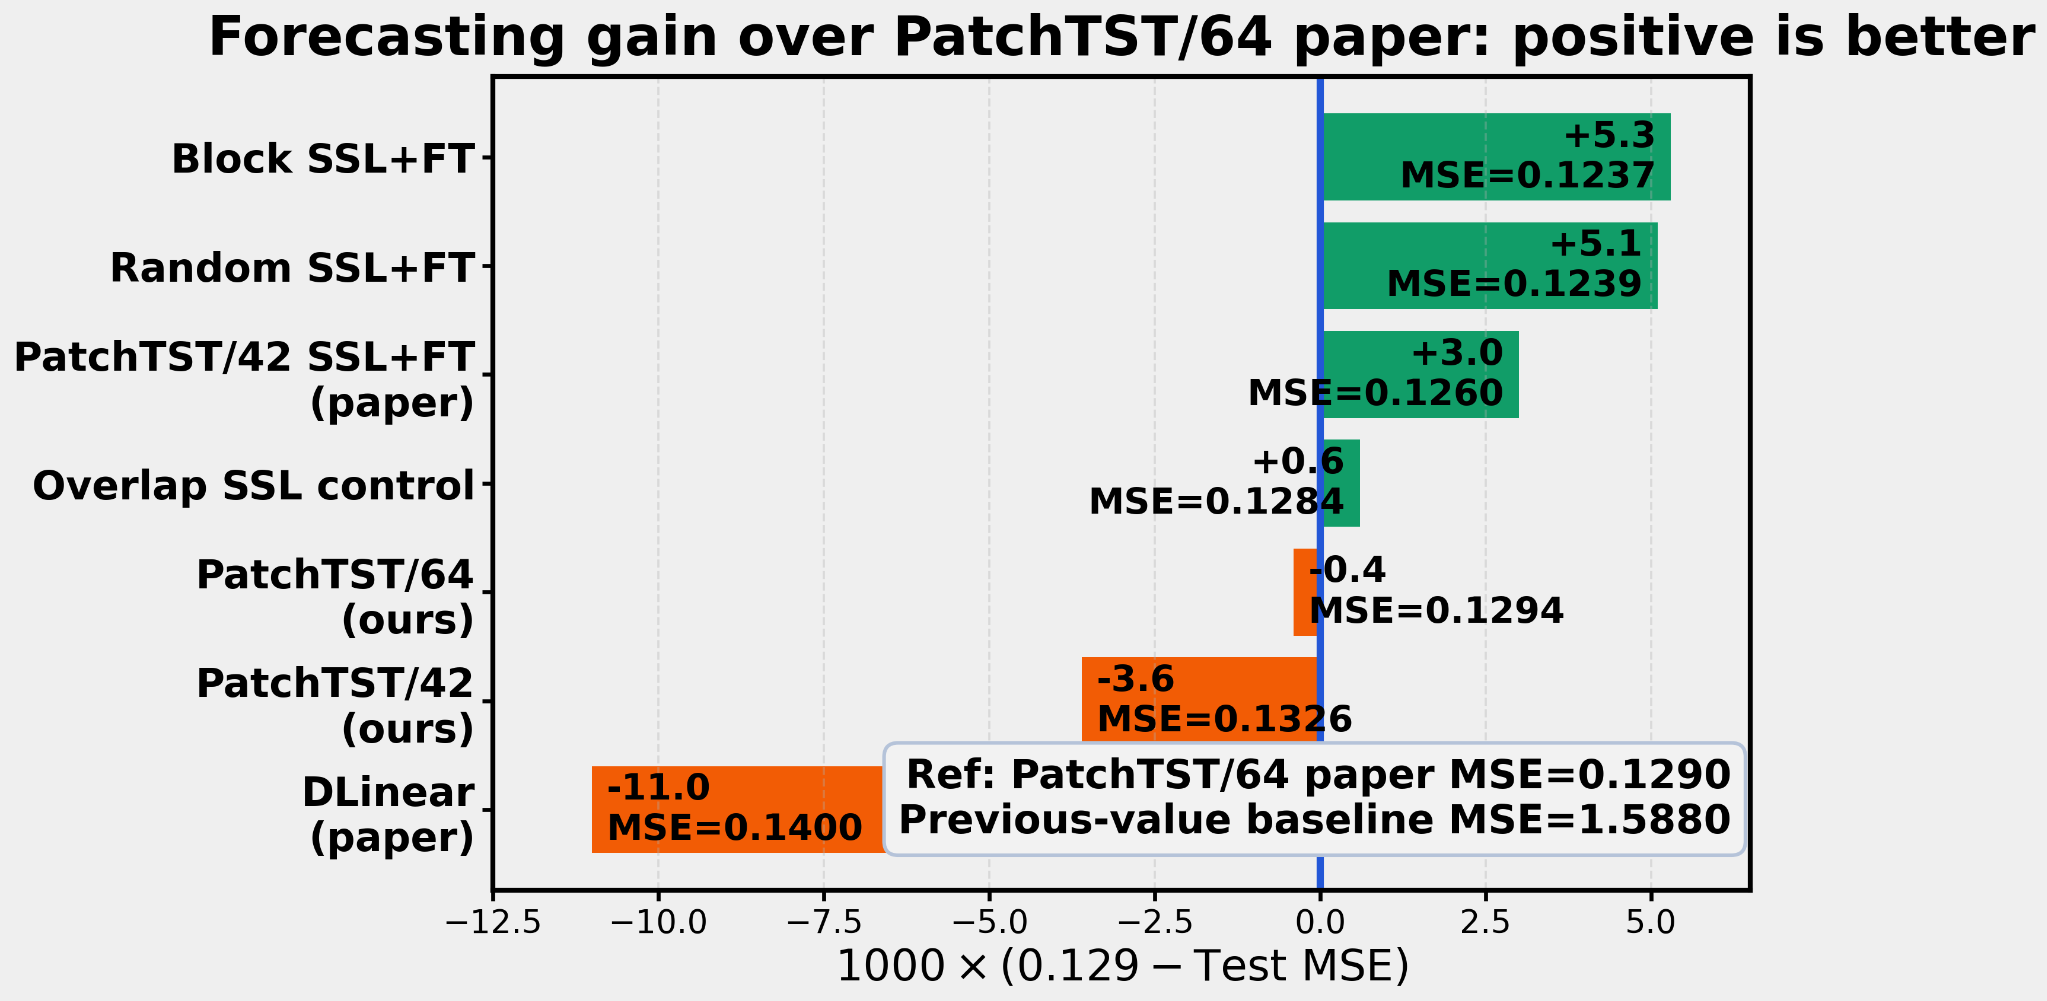
\includegraphics[width=\linewidth]{forecasting_gain_user.png}
\caption{Project result figure. Positive gain means lower MSE than the PatchTST/64 paper baseline.}
\label{fig:forecasting_gain}
\end{minipage}\hfill
\begin{minipage}{0.485\textwidth}
\centering
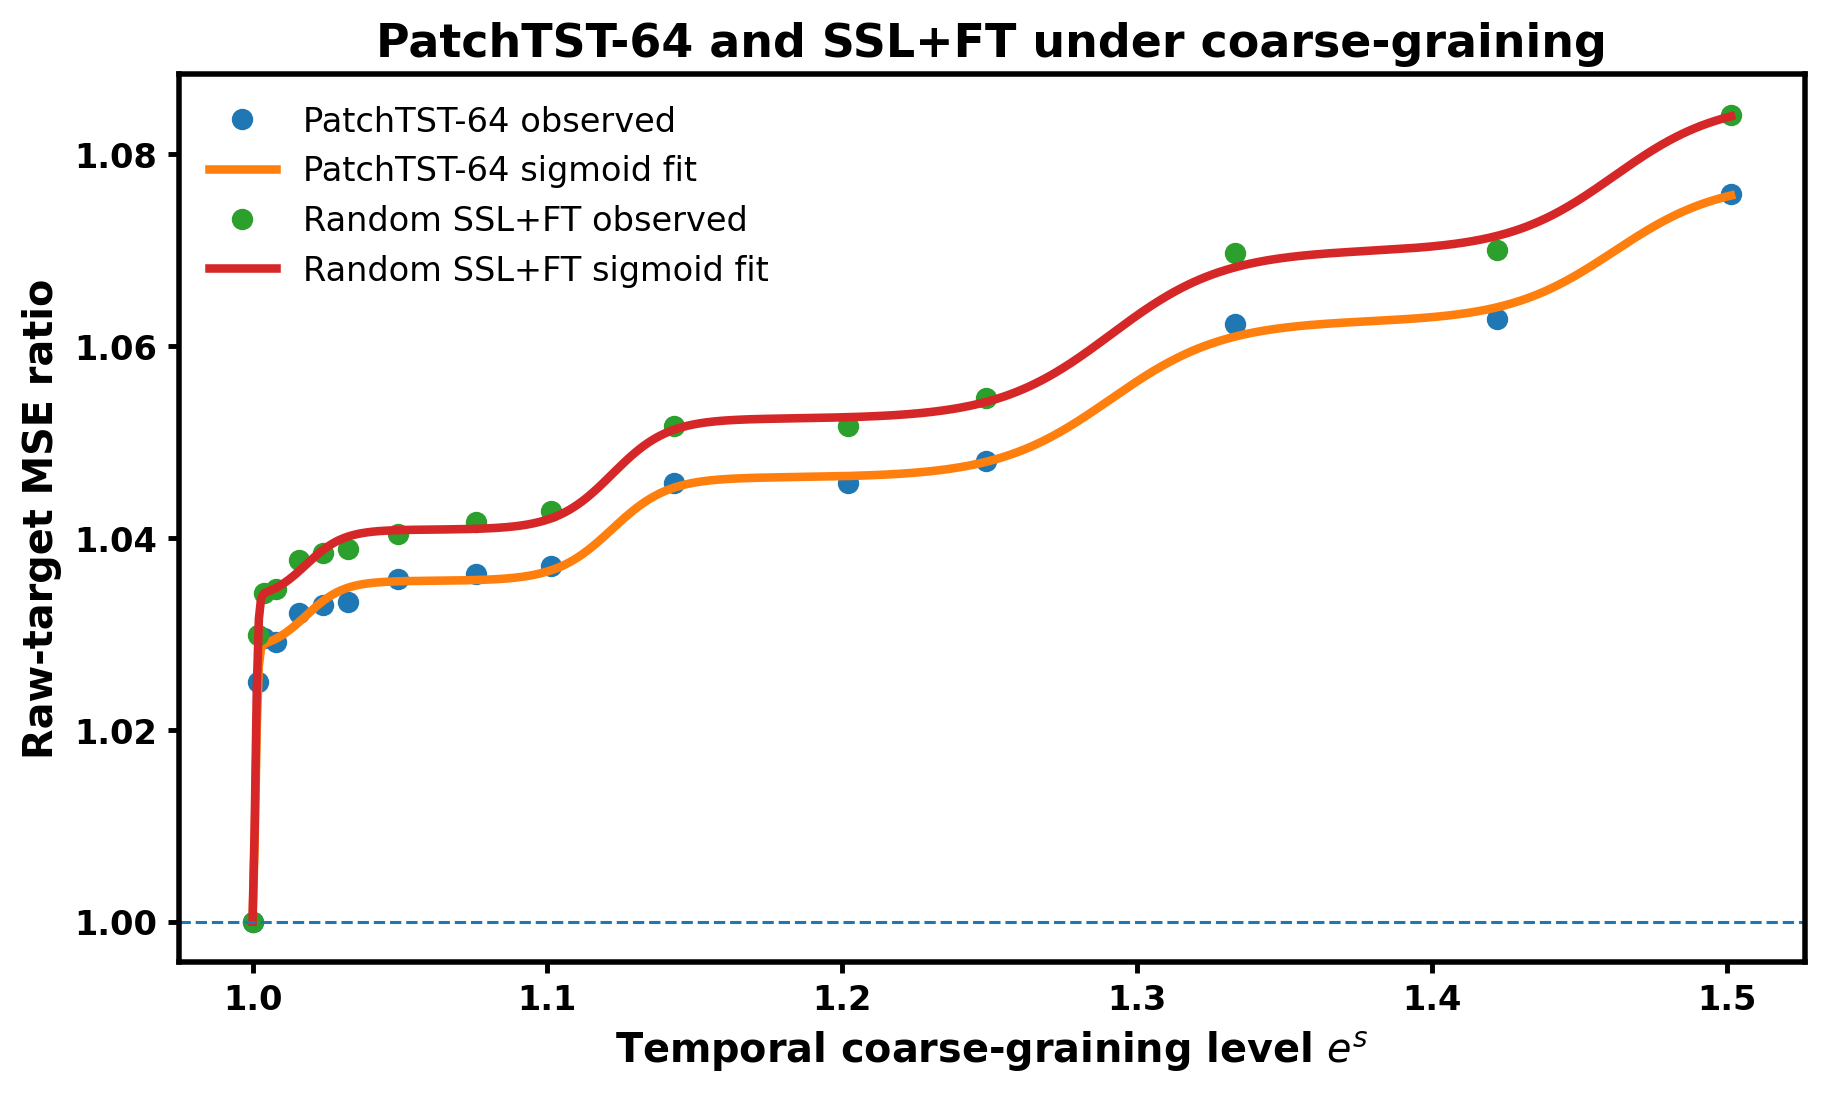
\includegraphics[width=\linewidth]{scale_sensitivity_user.png}
\caption{Scale probe. Higher raw-target MSE ratio means stronger degradation after coarse-graining.}
\label{fig:scale_sensitivity}
\end{minipage}
\end{figure}
\vspace{-1.3em}


\begin{table}[H]
\centering
\scriptsize
\caption{Complete numerical summary and experiment settings.}
\label{tab:complete_results}
\begin{tabular}{lcccccc}
\toprule
Method & $L$ & $H$ & $P$ & $S$ & pre/FT & Test MSE \\
\midrule
Previous-value baseline & 512 & 96 & -- & -- & 0/0 & 1.5880 \\
DLinear paper baseline & 512 & 96 & -- & -- & -- & 0.1400 \\
PatchTST/42 supervised & 336 & 96 & 16 & 8 & 0/30 & 0.1326 \\
PatchTST/64 paper reference & 512 & 96 & 16 & 8 & -- & 0.1290 \\
PatchTST/64 supervised & 512 & 96 & 16 & 8 & 0/30 & 0.1294 \\
Overlap SSL control & 336 & 96 & 16 & 8 & 30/15 & 0.1284 \\
Paper SSL fine-tuning & -- & 96 & -- & -- & -- & 0.1260 \\
Random SSL+FT & 512 & 96 & 12 & 12 & 30/15 & 0.1239 \\
Block SSL+FT & 512 & 96 & 12 & 12 & 30/10 & \textbf{0.1237} \\
\bottomrule
\end{tabular}
\end{table}

\end{document}
